\documentclass[tikz,border=5pt]{standalone}
\usepackage{amsmath}
\definecolor{curveblue}{HTML}{245C86}
\begin{document}
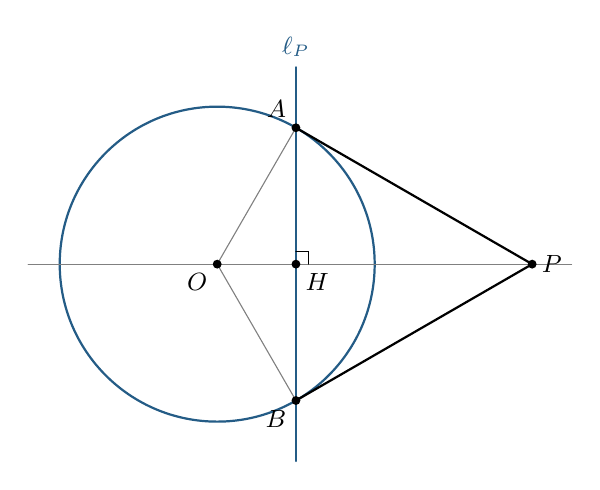
\begin{tikzpicture}[scale=2,font=\small,line cap=round]
\draw[curveblue,thick](0,0)circle(1);
\coordinate(O)at(0,0);\coordinate(P)at(2,0);\coordinate(A)at(.5,.866025);\coordinate(B)at(.5,-.866025);\coordinate(H)at(.5,0);
\draw[gray](-1.2,0)--(2.25,0);
\draw[thick](A)--(P)--(B);\draw[curveblue,thick](.5,-1.25)--(.5,1.25)node[above]{$\ell_P$};
\draw[gray](O)--(A) (O)--(B);
\foreach \N/\pos in {O/below left,P/right,A/above left,B/below left,H/below right}{\fill(\N)circle(.8pt)node[\pos]{$\N$};}
\draw(.5,.08)--(.58,.08)--(.58,0);
\end{tikzpicture}
\end{document}
